\chapter{Методика тестирования}

Одной из задач дипломного проекта является создание методики тестирования взаимодействия Flex приложения
с сервером. Методика должна в качестве основного инструмента тестирования использовать разработанный программный модуль.

Демонстрация методики осуществляется на примере тестирования Flex клиента, обладающего
несложным функционалом: клиент отправляет серверу запрос с указанными пользователем параметрами, а сервер отвечает
сообщением, в котором содержится переданная ему информация. На Рис.~\ref{ris:flexClient.png} изображён web-интерфейс приложения.

\begin{figure}[ht]
\center{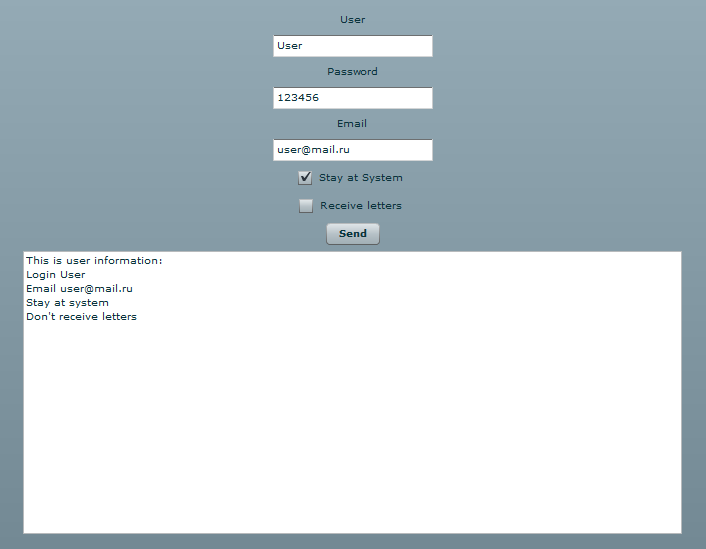
\includegraphics[height=70mm, width=100mm]{fig/development/flexClient.png}}
\caption{Web интерфейс Flex приложения}
\label{ris:flexClient.png}
\end{figure}

Пользователь указывает необходимые данные, нажимает кнопку "Send" и в текстовом поле снизу появляется
ответ сервера.

Сформулируем ряд требований к данному приложению.

Функциональные требования:

\begin{enumerate}
\item При отправке корректного запроса сервер должен отвечать сообщением, содержащим в себе следующие
данные введённые пользователем: User, Email, Stay at System/Don't stay at system, Receive letters/Don't
receive letters;
\item При отправке некорректного запроса сервер должен отвечать сообщением об ошибке с соответствующим
описанием.
\end{enumerate}

Требования к нагрузке:

\begin{enumerate}
\item Приложение должно выполнять свой функионал при работе с ним ста пользователей одновременно.
\end{enumerate}

На основании сформулированных функциональных и нагрузочных требований к приложению составлен план тестирования
и набор тестовых случаев.

\section{План тестирования}

\subsection{Объект тестирования}

Объектом тестирования является взаимодействие Flex клиента с сервером BlazeDS.

\subsection{Цели и приоритеты тестирования}

Целью тестирования является проверка соответствия программного обеспечения функциональным требованиям,
а также работоспособности программного обеспечения под заданной нагрузкой.

\subsection{Стратегии тестирования}

К тестированию приложения планируется применение следующих видов тестирования:

\begin{enumerate}
\item функциональное тестирование --- для проверки соответствия требованиям, указанным в техническом задании.
\item нагрузочное тестирование --- для проверки работоспособности ПО в заданных условиях.
\end{enumerate}

\subsection{Последовательность работ}

\begin{enumerate}
\item Проектирование набора тестовых случаев;
\item Подготовка тестового окружения;
\item Проведение тестирования;
\item Анализ результатов;
\end{enumerate}

\subsection{Критерии начала тестирования}

\begin{enumerate}
\item законченность разработки требуемого функционала;
\item покрытие кода тестируемого приложения юнит-тестами;
\item наличие задокументированных требований к программному обеспечению;
\item наличие набора тестовых случаев;
\item готовность тестового окружения.
\end{enumerate}

\subsection{Критерии окончания тестирования}

\begin{enumerate}
\item соответствие продукта функциональным требованиям;
\item стабильность работы продукта под заданной нагрузкой;
\end{enumerate}

\subsection{Тестовое окружение}

Для проведения тестирования необходимо следующее программное обеспечение:

\begin{enumerate}
\item сервер BlazeDS;
\item Flex приложение;
\item web-браузер c установленным Flash Player;
\item Apache JMeter.
\end{enumerate}

\section{Набор тестовых случаев}

\subsection{Настройка тестового окружения}

Перед проведением тестов необходимо настроить тестовую среду следующим образом:

\begin{enumerate}
\item установить программное обеспечение, указанное в разделе "Тестовое окружение" плана приёмочных испытаний.
Место установки JMeter далее будем называть JMETER\_HOME;
\item подключить к JMeter тестируемый модуль amf-translator --- добавить jar-файл приложения в каталог
JMETER\_HOME/lib/ext;
\item развернуть Flex приложение на сервере BlazeDS;
\item запустить JMeter --- приложение запускается с помощью файла jmeter.bat или ApacheJMeter.jar, находящихся в
каталоге JMETER\_HOME/bin.
\end{enumerate}

\subsection{Функциональные тесты}

{\bfseries Проверка обработки корректного запроса приложения}

Предусловия:

\begin{enumerate}
\item Добавить в Test Plan группу потоков - Thread Group (Test Plan > Threads (Users) > Thread Group).

\begin{figure}[ht]
\center{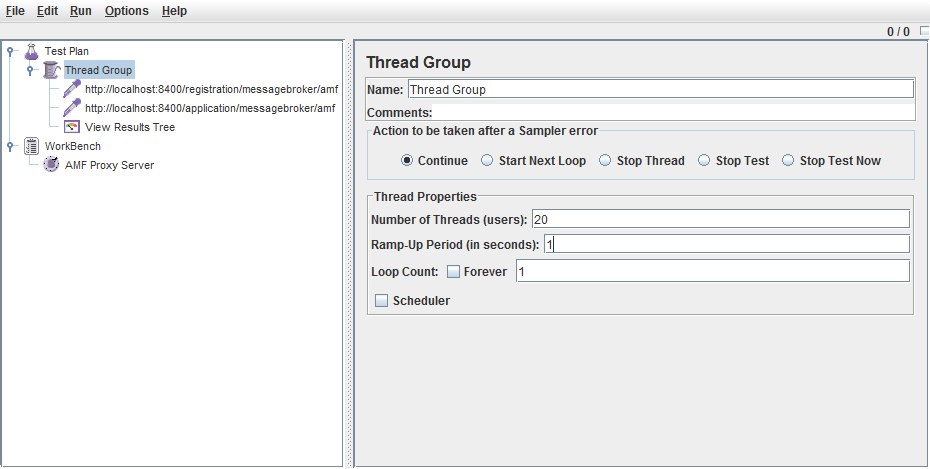
\includegraphics[height=80mm, width=120mm]{fig/development/testplan.png}}
\caption{Создание группы потоков}
\label{ris:testplan.png}
\end{figure}

\item Задать для Thread Group следующие параметры:

\begin{enumerate}
\item Действие, которое будут производиться в случае, если в тест выполняется с ошибкой
(Action to be taken after a Sampler error) --- Continue ;
\item число потоков, в которое будут запускаться шаги тест-плана (Number of Threads) установить равным единице;
\item Интервал, в течение которого будет запущено указанное в предыдущем параметре
число потоков (Ramp-Up Period) установить равным единице;
\item Число повторений набора тестов (Loop Count) установить равным единице;
\end{enumerate}

\item добавить визуалайзер результатов, чтобы иметь возможность отслеживать ход выполнения теста (Thread Group >
Add > Listener > View Results Tree)
\end{enumerate}

Шаги теста:

\begin{enumerate}
\item В Thread Group в качестве дочернего элемента добавить AMF RPC Sampler;
\item В AMF RPC Sampler записать верные параметры AMF запроса, а именно:
\begin{enumerate}
\item Endpoint Url - URL, по которому отправляется запрос;
\item AMF Call - имя удалённого объекта и процедуы(Например, если мы хоти вызвать у объекта registrationDestionation метод registerUser,
в этом поле следует написать registrationDestination.registerUser);
\item Request Parameters - параметры, в том порядке, в котором они должны быть переданы методу.
\end{enumerate}

\begin{figure}[ht]
\center{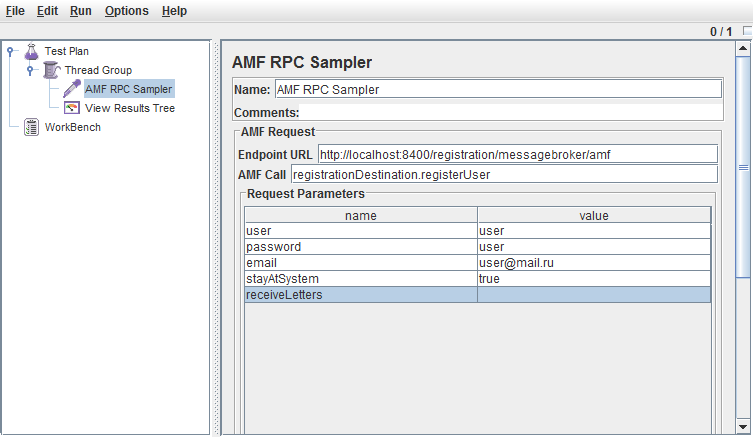
\includegraphics[height=80mm, width=120mm]{fig/development/amfSampler.png}}
\caption{Интерфейс элемента AMF RPC Sampler}
\label{ris:amfSampler.png}
\end{figure}

\item Запустить содержимое элемента Test Plan (Run > Start);
\end{enumerate}

Ожидаемый результат:

\begin{enumerate}
\item После завершения прогона тестов во View Results Tree в дереве элементов тест плана элемент AMF RPC Sampler
посдвечен зелёным цветом (сервер обработал запрос и не прислал сообщений об ошибке);
\item во вкладке Response Data элемента View Results Tree отображается сообщение сервера, соответствующее
переданным параметрам.
\end{enumerate}

\begin{figure}[ht]
\center{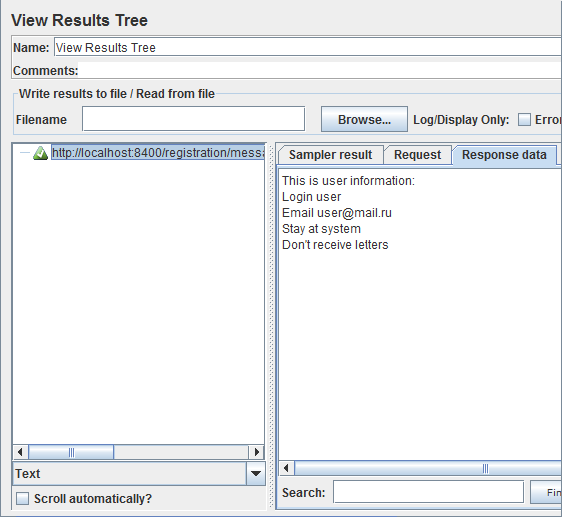
\includegraphics[height=80mm, width=120mm]{fig/development/positiveTest.png}}
\caption{Результаты корректного теста}
\label{ris:positiveTest.png}
\end{figure}

{\bfseries Проверка отправки некорректного AMF запроса}

Предусловия:

\begin{enumerate}
\item Добавить в Test Plan группу потоков - Thread Group (Test Plan > Threads (Users) > Thread Group).
\item Задать для Thread Group следующие параметры:

\begin{enumerate}
\item Действие, которое будут производиться в случае, если в тест выполняется с ошибкой
(Action to be taken after a Sampler error) --- Continue ;
\item число потоков, в которое будут запускаться шаги тест-плана (Number of Threads) установить равным единице;
\item Интервал, в течение которого будет запущено указанное в предыдущем параметре
число потоков (Ramp-Up Period) установить равным единице;
\item Число повторений набора тестов (Loop Count) установить равным единице;
\end{enumerate}

\item добавить визуалайзер результатов, чтобы иметь возможность отслеживать ход выполнения теста (Thread Group >
Add > Listener > View Results Tree)
\end{enumerate}

Шаги теста:

\begin{enumerate}
\item В Thread Group в качестве дочернего элемента добавить AMF RPC Sampler;
\item Ввести в AMF RPC Sampler неверное имя метода удалённого объекта и запустить содержимое элемента Test Plan (Run > Start);
\end{enumerate}

Ожидаемый результат:

\begin{enumerate}
\item После завершения прогона тестов во View Results Tree в дереве элементов тест плана элемент AMF RPC Sampler
подсвечен красным цветом (тест не пройден);
\item Ответ сервера во вкладке View Results Tree должен содержать сообщение о соответсвующей ошибке.

\begin{figure}[ht]
\center{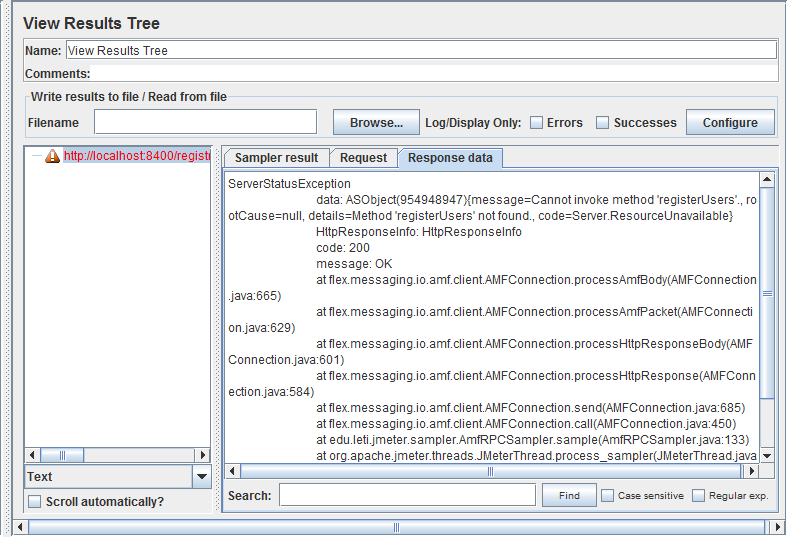
\includegraphics[height=80mm, width=120mm]{fig/development/negativeTest.png}}
\caption{Результаты некорректного теста}
\label{ris:negativeTest.png}
\end{figure}

\end{enumerate}

\subsection{Нагрузочные тесты}

{\bfseries Проверка работоспособности приложения под заданной нагрузкой}

Предусловия:

\begin{enumerate}
\item Добавить элемент AMF Proxy Server (WorkBench > Add > Non-Test Elements > AMF Proxy Server);

\begin{figure}[ht]
\center{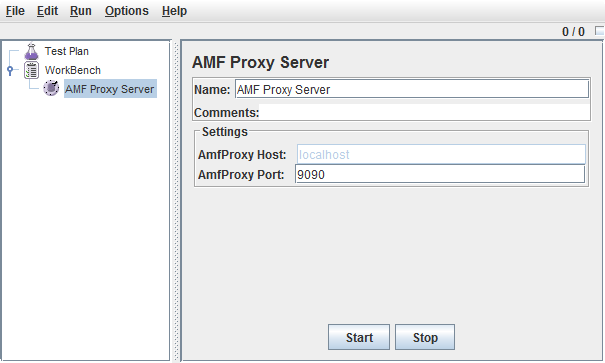
\includegraphics[height=80mm, width=120mm]{fig/development/proxySettings.png}}
\caption{Настройка прокси-сервера}
\label{ris:proxySettings.png}
\end{figure}

\item В поле AmfProxy Port необходимо указать номер порта, который будет слушать наш прокси сервер.
Если указать, например, 9090, то прокси-сервер будет запущен на localhost:9090;
\item Запустить браузер и указать там точно такие же настройки прокси-сервера.
Также стоит убедиться, что указанный Вами порт уже не занят другим приложением;
\item Запустить прокси-сервер, нажав кнопку "Start";
\item Далее открыть в браузере Flex приложение, и отправить пять-шесть запросов с корректными параметрами;
\item Завершить запись тестовых запросов, нажав кнопку "Stop";

\begin{figure}[ht]
\center{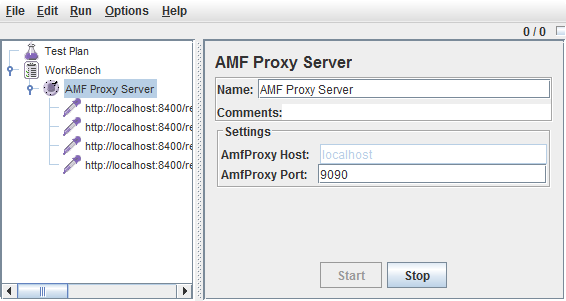
\includegraphics[height=80mm, width=120mm]{fig/development/proxyRequests.png}}
\caption{Запись запросов}
\label{ris:proxyRequests.png}
\end{figure}

\end{enumerate}

Шаги теста:

\begin{enumerate}
\item Добавить в Test Plan группу потоков - Thread Group (Test Plan > Threads (Users) > Thread Group).
\item Задать для Thread Group следующие параметры:

\begin{enumerate}
\item Действие, которое будут производиться в случае, если в тест выполняется с ошибкой
(Action to be taken after a Sampler error) --- Continue ;
\item число потоков, в которое будут запускаться шаги тест-плана (Number of Threads) установить равным 100 (
согласно требованиям к нагрузке на приложение);
\item Интервал, в течение которого будет запущено указанное в предыдущем параметре
число потоков (Ramp-Up Period) установить равным единице;
\item Число повторений набора тестов (Loop Count) установить равным единице;
\item Задать расписание запуска тестов: время начала тестов и время окончания тестов должны отличаться на
шесть часов, продолжительность теста равна 21600 секундам, задержка --- одной секунде;

\begin{figure}[ht]
\center{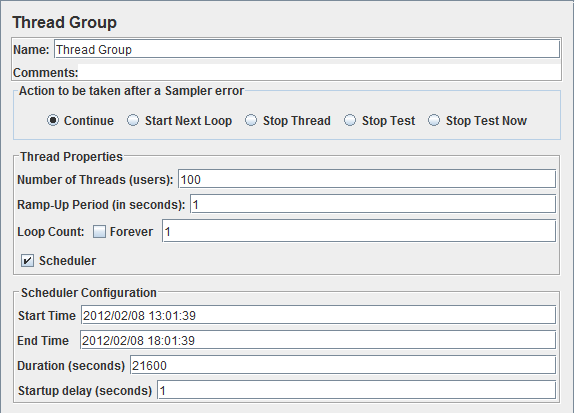
\includegraphics[height=80mm, width=120mm]{fig/development/threadParams.png}}
\caption{Настройки Thread Group}
\label{ris:threadParams.png}
\end{figure}

\end{enumerate}

\item перенести записанные с помощью AMF Proxy Server запросы в Test Plan
\item добавить визуалайзер результатов, чтобы иметь возможность отслеживать ход выполнения теста (Thread Group >
Add > Listener > View Results Tree)
\item Запустить тест план.
\end{enumerate}

Ожидаемый результат:

 После завершения прогона тестов во View Results Tree в дереве элементов все тесты должны быть пройдены ---
 корректный ответ от сервера должен быть получен для каждого элемента.

 \begin{figure}[ht]
\center{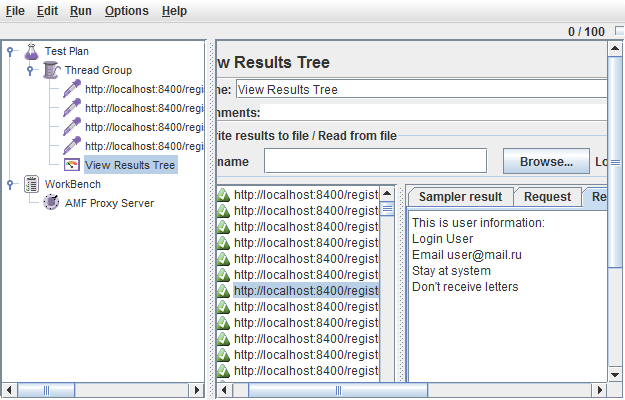
\includegraphics[height=80mm, width=120mm]{fig/development/load.png}}
\caption{Результаты нагрузочного тестирования}
\label{ris:load.png}
\end{figure}

Разработанная методика демонстрирует варианты использования реализованного программного модуля в
качестве инструмента тестирования взаимодействия Flex клиента с сервером. В частности в наборе
тестовых случаев были представлены примеры записи тестовых сценариев, отправка AMF запросов и
проверка результатов их выполнения, а также имитация работы с приложением большого числа пользователей
путём многопоточного запуска тестов.















